\documentclass{article}
\usepackage{
  amsmath, amsthm, amssymb, amsfonts,
  mathtools, xfrac, dsfont, mathrsfs, bm
  }
\usepackage{hyperref, float, parskip}
\usepackage[margin=0.8in]{geometry}
\usepackage[justification=centering,labelfont=bf]{caption}
\renewcommand{\arraystretch}{1.3}

% grouping and bookending
\newcommand{\pr}[1]{\left(#1\right)}
\newcommand{\br}[1]{\left[#1\right]}
\newcommand{\cbr}[1]{\left\{#1\right\}}
\newcommand{\floor}[1]{\left\lfloor#1\right\rfloor}
\newcommand{\ceil}[1]{\left\lceil#1\right\rceil}
\newcommand{\abs}[1]{\left|#1\right|}
\newcommand{\norm}[1]{\left\lVert#1\right\rVert}
\newcommand{\ip}[1]{\left\langle#1\right\rangle}
\renewcommand{\vec}[1]{\left\langle#1\right\rangle}
% derivatives
\newcommand{\der}[2]{\frac{d #1}{d #2}}
\newcommand{\mder}[2]{\frac{D #1}{D #2}}
\newcommand{\pder}[2]{\frac{\partial #1}{\partial #2}}
% common bold and script letters
\newcommand{\C}{\mathbb{C}}
\newcommand{\E}{\mathbb{E}}
\newcommand{\F}{\mathcal{F}}
\newcommand{\G}{\mathcal{G}}
\renewcommand{\L}{\mathscr{L}}
\newcommand{\N}{\mathbb{N}}
\renewcommand{\O}{\mathcal{O}}
\renewcommand{\P}{\mathbb{P}}
\newcommand{\Q}{\mathbb{Q}}
\newcommand{\R}{\mathbb{R}}
\renewcommand{\S}{\mathbb{S}}
\newcommand{\Z}{\mathbb{Z}}
% math operators
\DeclareMathOperator{\Cov}{Cov}
\DeclareMathOperator{\Var}{Var}
\let\Re\relax
\DeclareMathOperator{\Re}{Re}
\let\Im\relax
\DeclareMathOperator{\Im}{Im}
\DeclareMathOperator{\diag}{diag}
\DeclareMathOperator{\tr}{tr}
\DeclareMathOperator*{\argmax}{arg\,max}
\DeclareMathOperator*{\argmin}{arg\,min}
% misc
\newcommand{\mat}[1]{\begin{bmatrix}#1\end{bmatrix}}
\newcommand{\ind}[1]{\mathds{1}_{#1}}
\renewcommand{\epsilon}{\varepsilon}

\setlength\parindent{0pt}

\title{High Performance Computing: Final Project Proposal}
\author{Paul Beckman, Mariya Savinov}
\date{March 28, 2022}

\begin{document}

\maketitle

We would like to implement and test the parallelization of tree code \cite{barnes1986hierarchical} / fast multipole methods \cite{greengard1987fast} for the rapid evaluation of the total potential for a collection of particles interacting through a conservative force, e.g. the electrostatic potential for a collection of point charges. As a brief exposition of the problem, consider points $x_1, ..., x_n \in [0,1] = I$ with charges $q_1, ..., q_n$. We limit the positions to a one-dimensional problem so that we can focus on computational aspects, but imagine we are embedded in $\R^3$ so that the potential at $x$ of a particle at point $x_j$ with unit charge is
\begin{equation}
  \phi(x) = \frac{C}{\abs{x-x_j}}.
\end{equation}
where $C$ is some scaling factor (e.g. the Coulomb constant) which we will take to be $C=1$. We would like to evaluate the potential
\begin{equation}
  u(x_i) = \sum_{j=1}^n q_j \phi(\abs{x_i - x_j}) = \sum_{j=1}^n \dfrac{q_j}{\abs{x_i-x_j}}
\end{equation}
for each $x_i$, which in practice one would then use to compute forces between particles. The tree code / fast multipole idea is to hierarchically partition the interval $[0,1]$ using a binary tree, and accurately approximate
\begin{equation}
  u_k(x_i) = \sum_{x_j \in I_k} q_j \phi(\abs{x_i - x_j})
\end{equation} for all subintervals $I_k$ sufficiently far from $x_i$ by representing $\phi$ with its truncated Taylor series. One then repeats this computation for various levels in the hierarchy.

The primary computational questions involve the efficient distribution of the hierarchical data structure and computations across processes. We plan to approach these questions through the following tasks
\begin{itemize}
  \item Implement a serial $\O(n\log n)$ Barnes-Hut type tree-code
  \item Parallelize this approach using OpenMP, experimenting with tuning for improved cache usage
  \item Parallelize this approach using MPI, experimenting with communication minimization between cores
  \item (If time allows) improve tree code to an $\O(n)$ fast multipole method and modify parallelism accordingly
\end{itemize}

\begin{figure}
  \centering
  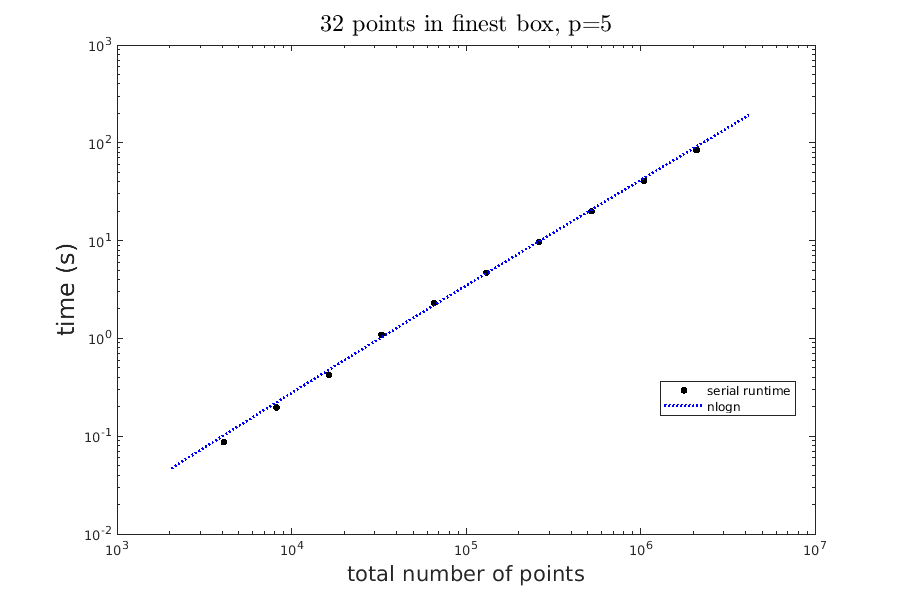
\includegraphics[width=0.55\textwidth]{./figures/varying_n_m32_p5.png}
\end{figure}

\begin{figure}
  \centering
  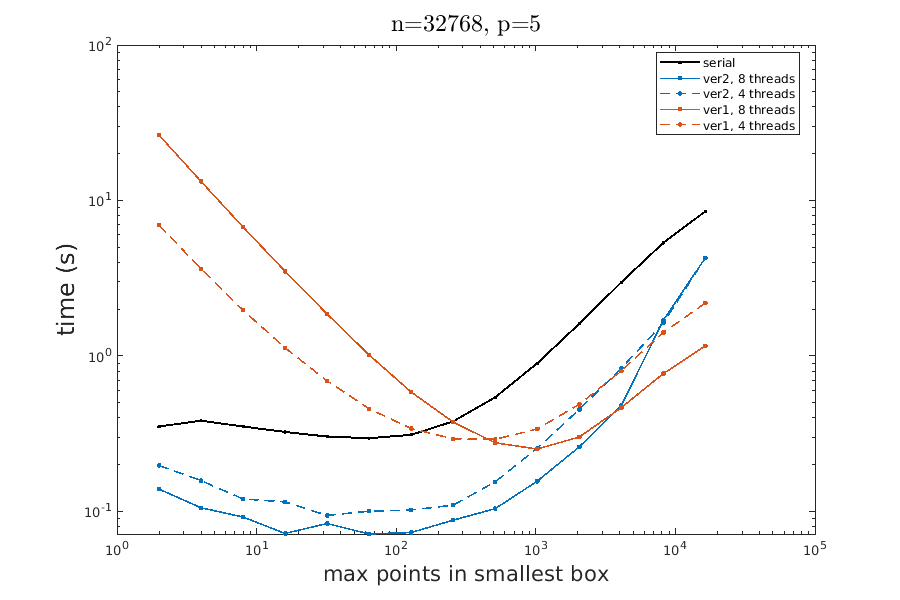
\includegraphics[width=0.55\textwidth]{./figures/varying_m_n32768_p5_4_8.png}
\end{figure}

\begin{figure}
  \centering
  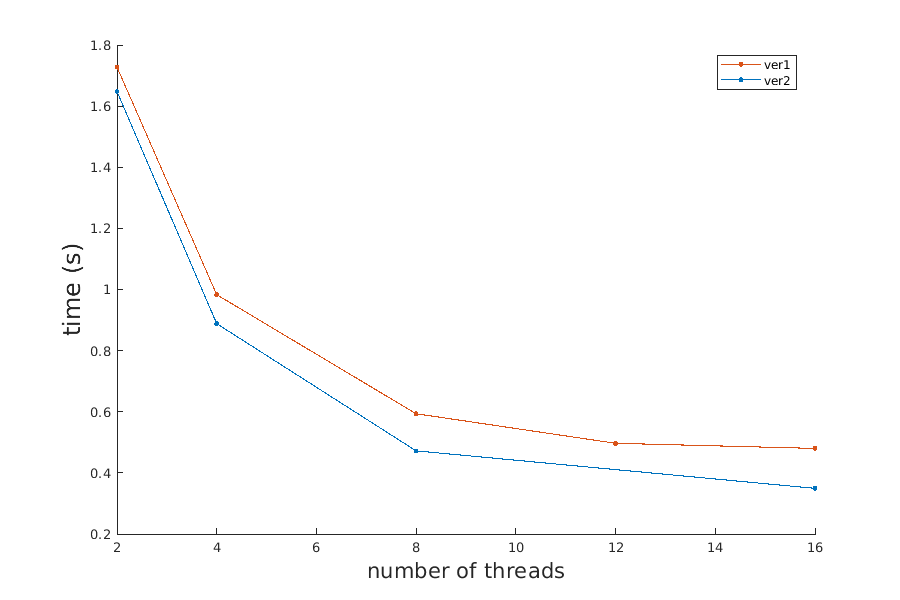
\includegraphics[width=0.45\textwidth]{./figures/strong_scalability.png} %
  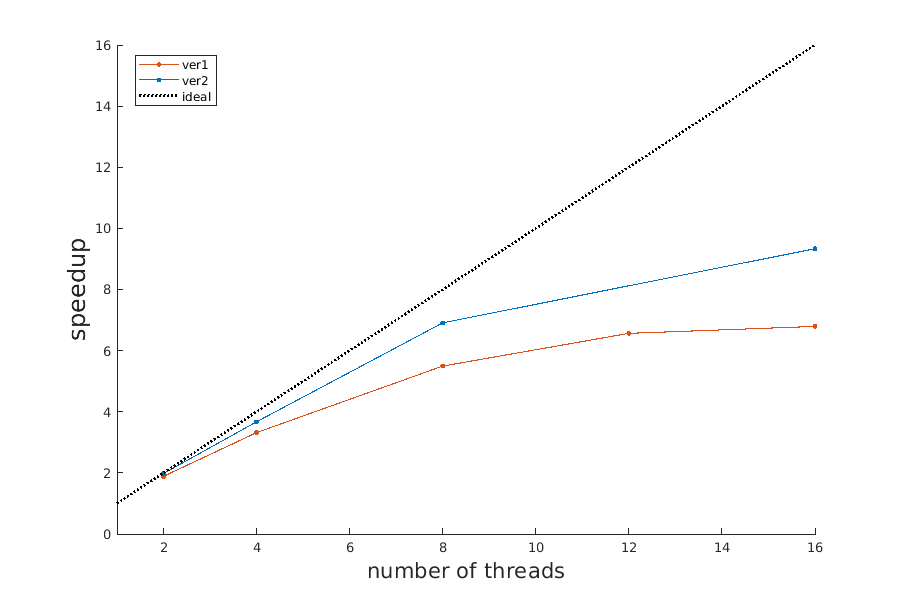
\includegraphics[width=0.45\textwidth]{./figures/strong_scalability2.png} 
\end{figure}

\begin{figure}
  \centering
  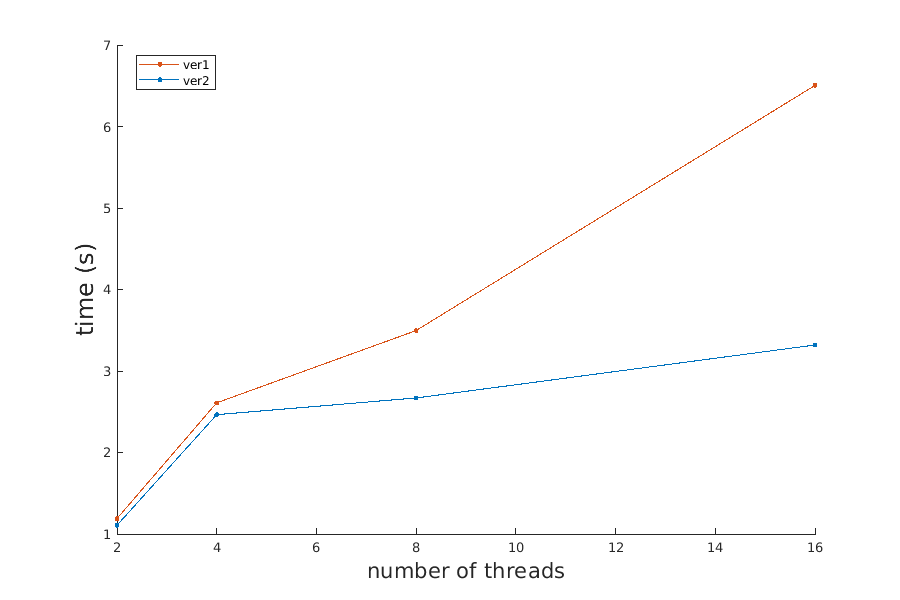
\includegraphics[width=0.45\textwidth]{./figures/weak_scalability.png} %
  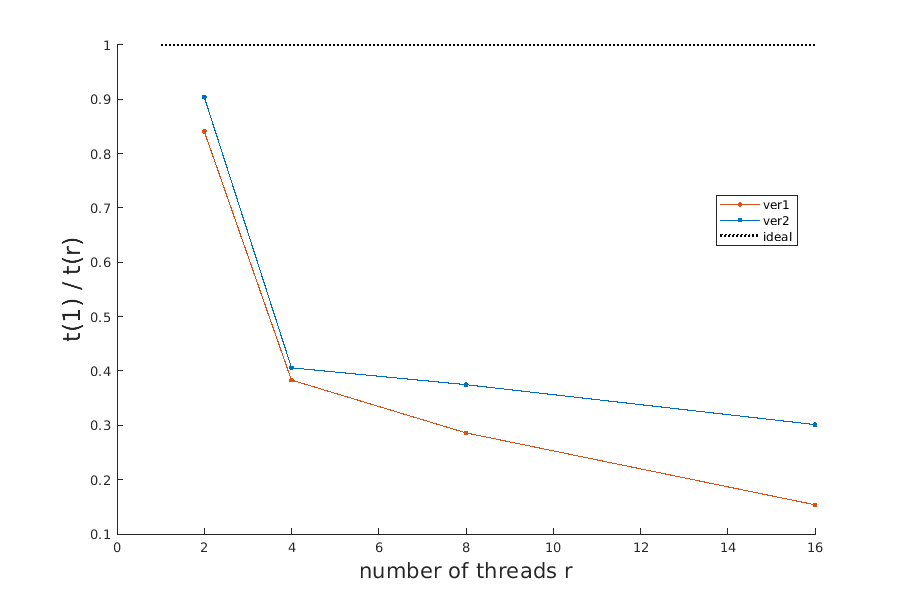
\includegraphics[width=0.45\textwidth]{./figures/weak_scalability2.png} 
\end{figure}

\bibliographystyle{plain}
\bibliography{refs}

\end{document}
